\documentclass[12pt]{article}
\usepackage{titling}
\usepackage{setspace}
\usepackage{hyperref}
\usepackage{lipsum}
\usepackage{graphicx}
\usepackage[margin=1in]{geometry}

\newcommand{\PutTitle}[1]
{
    \begin{center}
        {\huge\bfseries\thetitle}\\
        by \theauthor\\
        \thedate\\
        #1        
    \end{center}
    \hrule
    \vspace{2ex}
}

\setlength\paperwidth{8.5in}
\setlength\paperheight{11in}
\setlength\parindent{24pt}

\hypersetup
{
    colorlinks=true,
    linkcolor=blue,
    urlcolor=blue,
}

\begin{document}

\title{Title}
\author{Jonah Mondragon}
\date{\today}
\PutTitle{Period 6}

\doublespacing

% Description goes here as follows:
% Purpose:
% Procedures: (pictures/diagrams)
% Data/observations
% Conclusion: Problem, equation, statement (pictures/diagrams)

\begin{center}
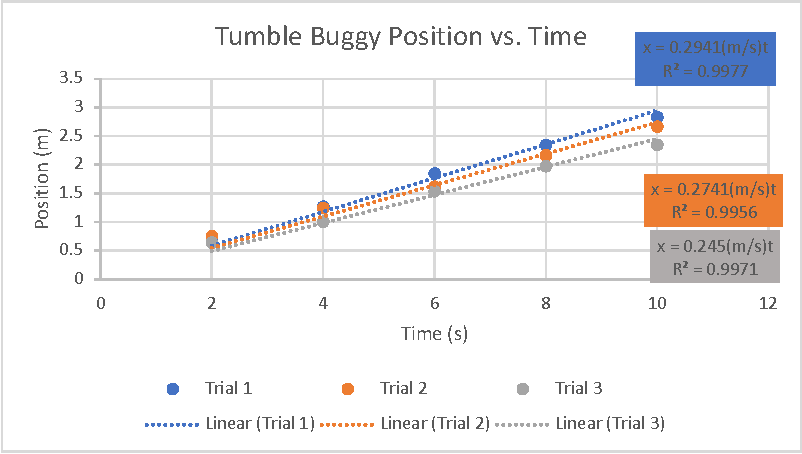
\includegraphics{tumble_buggy_position_vs_time_graph.pdf}
\end{center}

\end{document}

